\documentclass{beamer}
\usetheme{Warsaw}
\usepackage{wrapfig}
\title{Chatting with OTR over Tor with VPN}
\author{Gavin Bauer, Ryan McCarthy, Amruta Dubewar}
\date{\today}
\defbeamertemplate*{footline}{shadow theme}
{%
  \leavevmode%
  \hbox{\begin{beamercolorbox}[wd=.5\paperwidth,ht=2.5ex,dp=1.125ex,leftskip=.3cm plus1fil,rightskip=.3cm]{author in head/foot}%
    \usebeamerfont{author in head/foot}\insertframenumber\,/\,\inserttotalframenumber\hfill\insertshortauthor
  \end{beamercolorbox}%
  \begin{beamercolorbox}[wd=.5\paperwidth,ht=2.5ex,dp=1.125ex,leftskip=.3cm,rightskip=.3cm plus1fil]{title in head/foot}%
    \usebeamerfont{title in head/foot}\insertshorttitle%
  \end{beamercolorbox}}%
  \vskip0pt%
}
\begin{document}
\begin{frame}
\maketitle
\end{frame}
\section{VPN}
\subsection{Seting up the VPN}
\begin{frame}
\frametitle{Setting up the VPN}
\begin{itemize}
\item Hello world
\end{itemize}
\end{frame}
\subsection{Checking connection}
\begin{frame}
\frametitle{Checking connection}
\begin{itemize}
\item Hello moto
\end{itemize}
\end{frame}
\section{Tor}
\subsection{Setting up Tor}
\begin{frame}
\frametitle{Last slide}
\begin{itemize}
\item Good by
\end{itemize}
\end{frame}
\subsection{Verifying Tor}
\begin{frame}
\frametitle{Last slide}
\begin{itemize}
\item Good by
\end{itemize}
\end{frame}
\section{Pidgin}
\subsection{How Pdigin Integrates}
\begin{frame}
\frametitle{How Pidgin Integrates}
\begin{itemize}
\item Pidgin (any others) has built-in proxy utility
\item All traffic is piped through proxy
\item Then traffic is routed to .onion server
\item Then traffic is forwarded to XMPP server
\end{itemize}
\end{frame}
\subsection{Setting up Pidgin}
\begin{frame}
\frametitle{Setting up Pidgin}
\begin{columns}
    \begin{column}{0.48\textwidth}
        \begin{itemize}
          \item Modify your account
          \item Go to Advanced
        \end{itemize}
    \end{column}
    \begin{column}{.5\textwidth}
        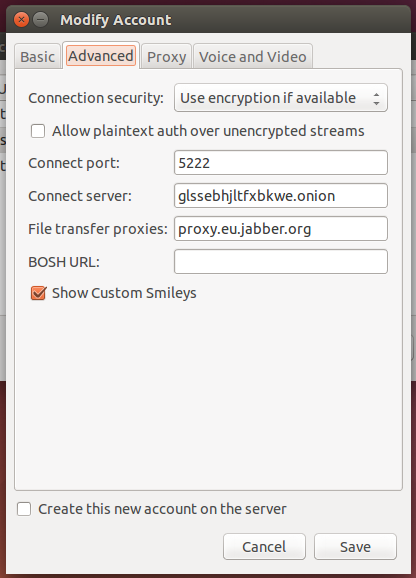
\includegraphics[width=.9\linewidth]{pidgin_advanced}
    \end{column}
\end{columns}
\end{frame}
\begin{frame}
\frametitle{Setting up Pidgin}
%\item Go to Advanced\\
\begin{columns}
    \begin{column}{0.48\textwidth}
        \begin{itemize}
          \item Go to Proxy
        \end{itemize}
    \end{column}
    \begin{column}{.5\textwidth}
        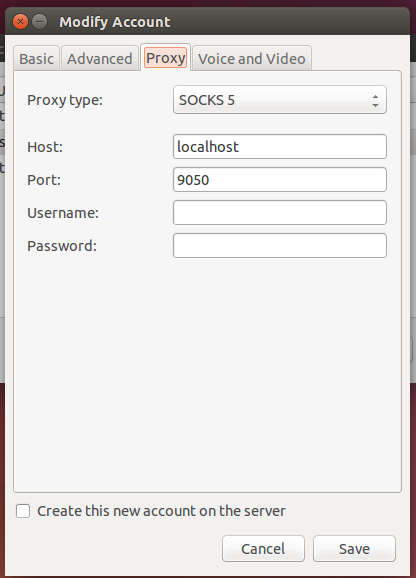
\includegraphics[width=.9\linewidth]{pidgin_proxy}
    \end{column}
\end{columns}
\end{frame}
\subsection{Verifying pdigin}
\begin{frame}
\frametitle{Verifying Pidgin}
\begin{columns}
    \begin{column}{0.48\textwidth}
        \begin{itemize}
          \item Login to the privacy box
          \item Attempt to OTR chat with someone
        \end{itemize}
    \end{column}
    \begin{column}{.5\textwidth}
        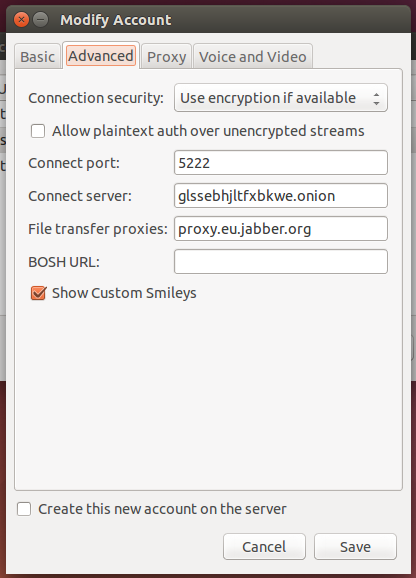
\includegraphics[width=.9\linewidth]{pidgin_advanced}
    \end{column}
\end{columns}
\end{frame}
\section{Summery}
\begin{frame}
\frametitle{Summery}
\begin{center}
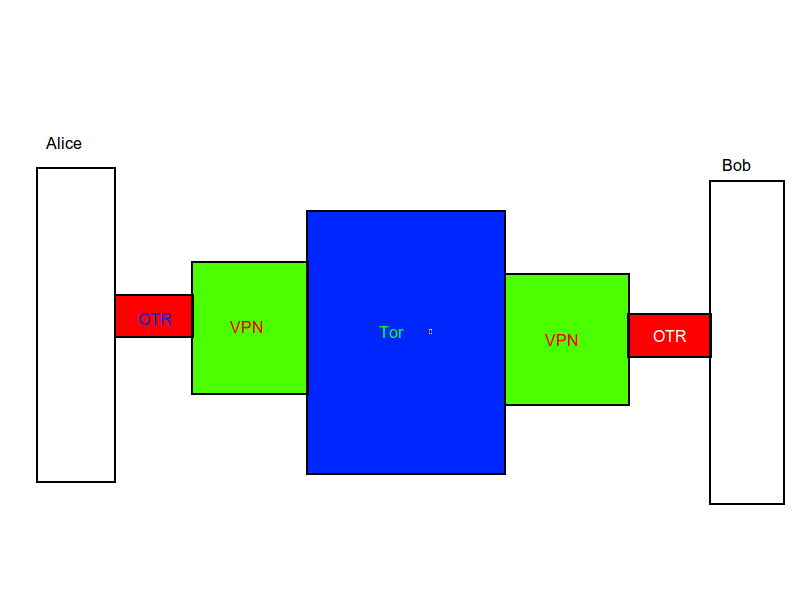
\includegraphics[width=1\linewidth]{overview}
\end{center}
\end{frame}
\section{Fin}
\end{document}
